\chapter{Related Work}
\label{ch:related_work}
This chapter outlines previous work by other researchers that is relevant to this thesis, supplementing the background information provided in Ch.~\ref{ch:background}. It primarily includes work on tutorial design and teaching through games.

\section{Tutorial Design}
\label{sec:tutorial_design}
Tutorials, as described in Sect.~\ref{sec:tutorials}, are widely used to teach users how to work with software products, among other things. With the tutorial, the creators aim to teach users how to perform various tasks with their tool, preferably in a \textbf{quick}, \textbf{intuitive}, \textbf{memorable}, and \textbf{error-free} way. Unfortunately, not all tutorial designs succeed in fulfilling all of these goals, but many efforts have been made to explore different approaches and improve on the standard tutorial design. Some of these are briefly described in the following sections.

\subsection{Stencils-Based Tutorials}
\label{sec:stencils}
The authors of the paper \emph{Stencils-Based Tutorials: Design and Evaluation}~\cite{kelleher:stencils} identify some problems with traditional tutorials: users may miss steps or perform actions that were not intended, and it is often difficult to find the components described in the tutorial.

\noindent
In their work, the authors introduce \emph{Stencils}, which is an alternative way of presenting a tutorial by adding a translucent colored interface layer on top of the original \gls{ui}, with holes highlighting the relevant elements, as seen in Fig.~\ref{fig:stencils}. Additionally, tutorial information is displayed on this layer in the form of sticky notes.

\begin{figure}[htp]
	\centering
	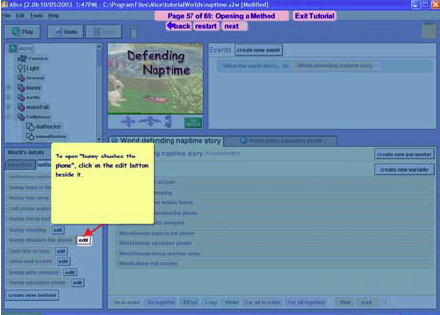
\includegraphics[scale=0.70]{stencils}
	\caption[\emph{Stencils} example]{An example of highlighting relevant \gls{ui} elements with \emph{Stencils} through holes in the colored layer. Tutorial information is added with the yellow sticky note. \emph{Image source:~\cite{kelleher:stencils}}}
	\label{fig:stencils}
\end{figure}

\noindent
With the results of a user study, the authors show that with a \emph{Stencils}-based tutorial, users were able to complete tutorials faster, with fewer errors and less human assistance. They also note that their tutorial approach can likely be improved by decreasing the level of assistance depending on the users familiarity with the system. A need for tutorial tasks that are directly relevant to the users, as opposed to ``artificial'' tutorial exercises, is also mentioned.


\subsection{DocWizards}
\label{sec:docwizards}
The authors of the paper \emph{DocWizards: A System for Authoring Follow-me Documentation Wizards}~\cite{bergman:docwizards} identify that there are some problems with teaching people to use software (\emph{computer-based procedures}) through documentation alone. Users must find \gls{ui} elements based on documentation descriptions on their own, understand and handle conditional branches, and at the same time keep track of where they are in the process.

\noindent
In their work, they propose the use of a tutorial-like documentation process called \emph{follow-me documentation wizards}, an approach that combines the advantages of conventional wizards and documentation. With their approach, processes are automatically captured from demonstrations made by expert users, and made available to new users in the form of highlighting both text from the documentation (see Fig.~\ref{fig:docwizards}) as well as UI elements for each step.

\begin{figure}[htp]
	\centering
	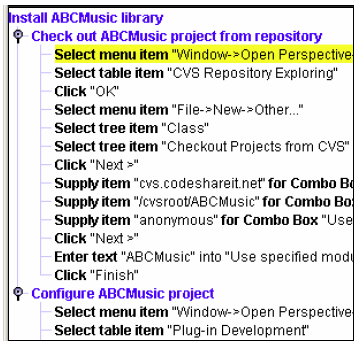
\includegraphics[scale=0.70]{docwizards}
	\caption[\emph{DocWizards} example]{An example of stepwise instructions in \emph{DocWizards}. The current step is highlighted in yellow. \emph{Image source:~\cite{bergman:docwizards}}}
	\label{fig:docwizards}
\end{figure}

\noindent
Finally, a user study is conducted by the authors to evaluate their system, yielding positive results. The usefulness of the \emph{DocWizards} approach has also been verified in a separate study~\cite{gweon:evaluating_docwizards}.

\subsection{Graphstract}
\label{sec:graphstract}
The authors of the paper \emph{Graphstract: Minimal Graphical Help for Computers}~\cite{huang:graphstract} identify problems with the commonly used approach of providing only a textual explanations in software tutorials and help. Users are unlikely to read these explanations carefully enough, if at all. Simply adding screenshots of the \gls{ui} is not an adequate solution, since these usually add far more information than necessary, and thus increase the perceived size and complexity of the explanation. Problems with animation and video are also identified, such as making it difficult for the user to move at their own pace.

\noindent
Instead of relying on text-only descriptions or simple screenshots, the authors propose the use of graphical help in the form of partial screenshots, combined to show a complete sequence of actions required to perform a task (see Fig.~\ref{fig:graphstract}). This approach provides graphical help directly mapped to the \gls{ui}, without adding a lot of extra information. Additionally, the whole sequence is presented in a small space, making it easy to get an overview.

\begin{figure}[htp]
	\centering
	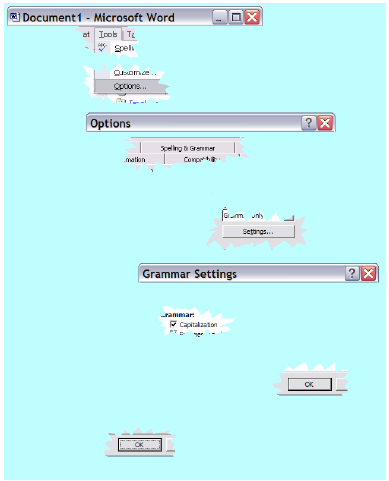
\includegraphics[scale=0.70]{graphstract}
	\caption[\emph{Graphstract} example]{An example of stepwise instructions in \emph{Graphstract} in the form of screenshot snippets, showing the steps required to toggle auto-capitalization in Microsoft Word. \emph{Image source:~\cite{huang:graphstract}}}
	\label{fig:graphstract}
\end{figure}

\noindent
Three iterations of user studies on a prototype is conducted by the authors, showing that \emph{Graphstract} performs better than conventional approaches overall, if not in all cases. They also conclude that adding text to the images is useful in many situations, despite their approach relying on graphical help only.

\subsection{Photo Tutorials}
\label{sec:photo_tutorials}
The authors of the paper \emph{Generating Photo Manipulation Tutorials by Demonstration}~\cite{grabler:photo_tutorials} argue the use of static visual tutorials (stepwise text-based tutorials accompanied by graphics) over video-tutorials for image processing software.

\noindent
In their work, the authors design a system for auto-generating static visual tutorials for a specific software product. These tutorials provide stepwise instructions with screenshots for completing a particular task, and additionally highlight the parts of the screenshots that are relevant to this task, as seen in Fig~\ref{fig:photo_tutorials}. This is combined with macros for automatic image labeling, to identify important regions of the particular image the user is working with.

\begin{figure}[htp]
	\centering
	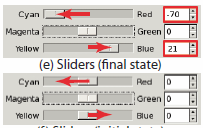
\includegraphics[scale=0.70]{photo_tutorials}
	\caption[\emph{Photo Tutorials} example]{An example of highlighting relevant \gls{ui} elements in a screenshot with \emph{Photo Tutorials}. \emph{Image source:~\cite{grabler:photo_tutorials}}}
	\label{fig:photo_tutorials}
\end{figure}

\noindent
Through a user study, the authors verify the effectiveness of their tutorials by observing that users perform significantly better and make less errors compared to tutorials based on text and video. However, some problem areas are identified: better tutorials can be created by providing feedback to users as they are performing the steps of the tutorial.

\subsection{Toolclips}
\label{sec:toolclips}
The authors of the paper \emph{ToolClips: An Investigation of Contextual
Video Assistance for Functionality Understanding}~\cite{grossman:toolclips} explore the \emph{learnability} of software products, more specifically relating to the concept of \emph{understanding} how to properly use functionality (see~\cite{grossman:software_learnability}). They identify problems with existing approaches based on both text and videos, where information is provided outside the context of the \gls{ui} in question. The authors also assess that regular tooltips, which provide the user with a short in-context description of what a \gls{ui} element does, do not provide a sufficient level of detail for complex tools.

\noindent
Attempting to provide the best of several worlds, the authors suggest their \emph{ToolClips} approach, enhancing regular tooltips with additional documentation and video content, in a more context-sensitive manner, as seen in Fig.~\ref{fig:toolclips}.

\begin{figure}[htp]
	\centering
	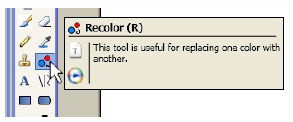
\includegraphics[scale=0.80]{toolclips}
	\caption[\emph{ToolClips} example]{An example of a \emph{ToolClip}, appearing as a regular tooltip, but with buttons allowing access to additional media. \emph{Image source:~\cite{grossman:toolclips}}}
	\label{fig:toolclips}
\end{figure}

\noindent
Through the results of two user studies, the authors show that the \emph{ToolClips} approach significantly improves users' understanding of how to use elements, and additionally has a positive impact on retention of this understanding, for applications that are \emph{highly graphical}.

\section{Learning With Games}
\label{sec:learning_with_games}
Most video games require the player to learn something in order to complete the game, whether it is difficult concepts like solving obscure puzzles, or simply the controls of the game. In some cases, games are even used to teach concepts for educational purposes, such as programming. In other cases, games even teach players valuable real-life skills without being deliberately designed to do so. The following sections briefly describe some of the efforts previously made in the field of educational games.

\subsection{Karel the Robot}
\label{sec:karel_the_robot}
Karel the Robot~\cite{pattis:karel_the_robot} is a game-like programming language and environment designed to teach basic programming concepts to beginners. It was developed by Richard E. Pattis in 1981, who used Karel to teach programming courses at Stanford University.

\noindent
The motivation behind Karel was to be able to teach students the basics programming without having to worry about the more complex and less important (to beginners) details. In Pattis' own words: \emph{``The careful omission of variables and data structures from Karel's language ... allows the immediate exploration of the rich domain of abstraction and control structures.''}~\cite{pattis:karel_the_robot}. This allows students to focus on learning how to solve problems through programming concepts.

\noindent
Karel was originally designed as a Pascal-like procedural programming language, but the concept gained wide popularity, and has been extended to Java~\cite{roberts:karel_the_robot_java},
Python\footnote{\url{http://gvr.sourceforge.net/}}$^{,}$\footnote{\url{https://code.google.com/p/rur-ple/}}, Karel++ (object-orientation)~\cite{bergin:karel_plus_plus}, REALbasic\footnote{\url{http://www.ohloh.net/p/rbkarel}}, and Scratch\footnote{\url{http://scratched.media.mit.edu/resources/karel-robot-scratch}}. Karel was inspired by the LOGO project\footnote{\url{http://el.media.mit.edu/logo-foundation/index.html}}, and has in turn inspired games like RoboMind.\footnote{\url{http://www.robomind.net/en/index.html}}

\noindent
The purpose of the game is to control a robot (Karel) by giving it a set of commands, and perform tasks. Initially, only a small set of commands are available, but as part of the learning process, users must learn how to extend these commands. The simplest task Karel is asked to perform is to pick up a beeper, seen as the diamond shape in Fig.~\ref{fig:karel_the_robot}.

\begin{figure}[htp]
	\centering
	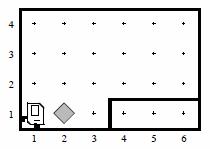
\includegraphics[scale=0.80]{karel_the_robot}
	\caption[Karel the Robot]{A simple \emph{Karel the Robot} level, where Karel (bottom left) must move to and pick up a single beeper (diamond shape). \emph{Image source:~\cite{roberts:karel_the_robot_java}}}
	\label{fig:karel_the_robot}
\end{figure}

\subsection{Josef the Robot}
\label{sec:josef_the_robot}
Josef the Robot~\cite{tomek:josef_the_robot} is a game-like programming environment similar to Karel (Sect.~\ref{sec:karel_the_robot}). Unlike Karel, Josef more closely resembles ``real'' programming languages by being rich in structures and operations. Like Karel, Josef is also inspired by the LOGO project.

\noindent
The author of Josef, Ivan Tomek, provides ample motivation for creating a more novice-friendly environment for learning how to program. Firstly, potential learners should find the problems they can solve with programming to be interesting, which is likely not the case (for the average person) with problems like sorting a sequence of numbers. Furthermore, novice programmers should not have to worry about the more complex rules that are not directly related to problem-solving, such as syntax and data handling.

\subsection{CodeSpells}
\label{sec:codespells}


\subsection{Serious Games}
\label{sec:serious_games}
Games that are designed for a purpose that is not pure entertainment are often called \emph{Serious Games}, a term likely popularized by The Serious Games Initiative\footnote{\url{http://www.seriousgames.org/}} in 2002~\cite{djaouti:serious_games}. This genre encompasses many different types of games, but a prime example of a serious game is the \emph{flight simulator}, a realistic type of game extensively used to teach pilots how to fly aircraft.

\noindent
Several organizations working with serious games exist. Some examples are the \emph{Serious Games Institute}\footnote{\url{http://www.seriousgamesinstitute.co.uk/}} the \emph{Games Learning Society}\footnote{\url{http://www.gameslearningsociety.org/}}, the \emph{Learning Games Network}\footnote{\url{http://learninggamesnetwork.org/}}, and \emph{Serious Games Interactive}\footnote{\url{http://www.seriousgames.net/}}.

\subsection{Kahoot}
Not relevant?

